\documentclass{article}
\usepackage[utf8]{inputenc}
\usepackage{geometry}
 \geometry{
 a4paper,
 total={170mm,257mm},
 left=20mm,
 top=20mm,
 }
 \usepackage{graphicx}
\usepackage{titling}
\usepackage{hyperref}
\usepackage{xcolor}

 \title{  Recommending Pairs of News Stories using Bandits 
}
\author{Gilles Callebaut}
\date{6/3/2025}

 
 \usepackage{fancyhdr}
\fancypagestyle{plain}{%  the preset of fancyhdr 
    \fancyhf{} % clear all header and footer fields
    \fancyhead[L]{Reinforcement Learning and Dynamic Optimization}
    \fancyhead[R]{\thedate}
    \fancyfoot[C]{\thepage}
}
\makeatletter
\def\@maketitle{%
  \newpage
  \null
  \vskip 1em%
  \begin{center}%
  \let \footnote \thanks
    {\LARGE \@title \par}%
    \vskip 1em%
    %{\large \@date}%
  \end{center}%
  \par
  \vskip 1em}
\makeatother

\usepackage{lipsum}
\usepackage{amsmath}
\usepackage{cmbright}

\begin{document}

\maketitle

\noindent\begin{tabular}{@{}ll}
     Student &  Michalis Lamprakis\\
     AM & 2020030077
\end{tabular}

\section*{Problem context}
Display a pair of articles $(i,j)$, 
where $i$ is placed on top and $j$ on bottom. 
The user clicks either $i$ (with probability $p_i$) or $j$
(with probability $(1-p_i)p_j$, but not both.
It is clear that the total expected reward is influenced by their joint configuration 
and given by the formula $p_i + (1-p_i)p_j$. So the goal is to
maximize the expected reward by selecting the best pair of articles.
So we made some slight modifications to our algorithms to fit the evironment.
\[
    \mu^*= p_i^* + (1-p_i^*)p_j^*
\]
\[
    \mu_{(i,j)} = p_i + (1-p_i)p_j 
\]
\[
    \Delta_{(i,j)} = \mu^* - \mu_{(i,j)}
\]

\noindent Implementantion of the assignment (In Google Colab): \\
\href{https://colab.research.google.com/drive/1S4G9UBfirLocYdTSE6vLyiHGKPBdcLDo?usp=sharing}{\textcolor{blue}{https://colab.research.google.com/drive/1S4G9UBfirLocYdTSE6vLyiHGKPBdcLDo?usp=sharing}}\\
The code contains detailed comments in which I explain everything.

\section*{Subtask 1}
In this task i made slight modifications to the given 
Explore \& Exploit code to fit the environment. 
Also, i implemented the UCB algorithm (i tried to follow the same structure
as the first algorythm). So the main difference here compared to a 
UCB algorithm for single-arm bandits is that when a pair $(i,j)$ is selected,
we update the statistics ($\hat{\mu}_{i}(t)$ and $N_i(t)$) for both arms no 
matter which one was clicked. This is because the reward is a function of both arms.\\\\
In the UCB algorithm i use o formula to calculate
the mean reward {$\hat{\mu}_{i}$} when a new reward is recieved. 
Here is the proof of this:\\\\
1. The current $\hat{\mu}_{i}$ after $n$ selections:
\[
    \hat{\mu}_{n} = \frac{r_1+r_2+...r_n}{n}
\]
2. When a new reward $r_{n+1}$ is recieved, the new $\hat{\mu}_{n+1}$ is:
\[
    \hat{\mu}_{n+1} = \frac{r_1+r_2+...r_n+r_{n+1}}{n+1}=
    \frac{n\hat{\mu}_{n}+r_{n+1}}{n+1}
\]
3. We substract $\hat{\mu}_{n}$ from both sides:
\[
    \hat{\mu}_{n+1} - \hat{\mu}_{n} = \frac{n\hat{\mu}_{n}+r_{n+1}}{n+1} - \hat{\mu}_{n}=
    \frac{n\hat{\mu}_{n}+r_{n+1} - (n+1)\hat{\mu}_{n}}{n+1}=
    \frac{r_{n+1} - \hat{\mu}_{n}}{n+1} \Rightarrow
    \boxed{\hat{\mu}_{n+1} = \hat{\mu}_{n} + \frac{r_{n+1} - \hat{\mu}_{n}}{n+1}}
\]  

\newpage

\noindent {\bf Results}:\\
\noindent After implementing the two algorithms, we 
plot the accumulated rewards for both of them, comparing them to 
the optimal reward (the reward achieved by displaying only the optimal pair).

\begin{figure}[h!]
    \centering
    \begin{minipage}{0.45\textwidth}
        \centering
        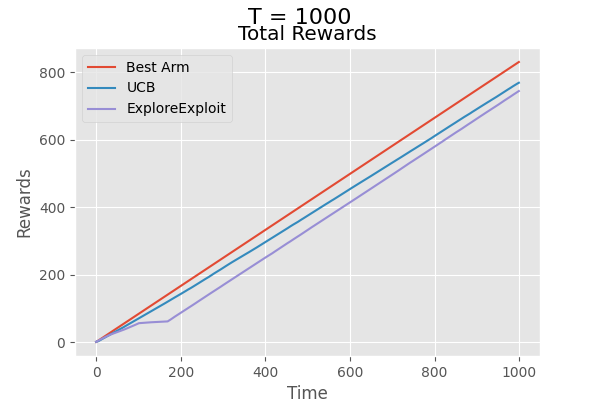
\includegraphics[width=\textwidth]{./Images/plot2.png}
    \end{minipage}\hfill
    \begin{minipage}{0.45\textwidth}
        \centering
        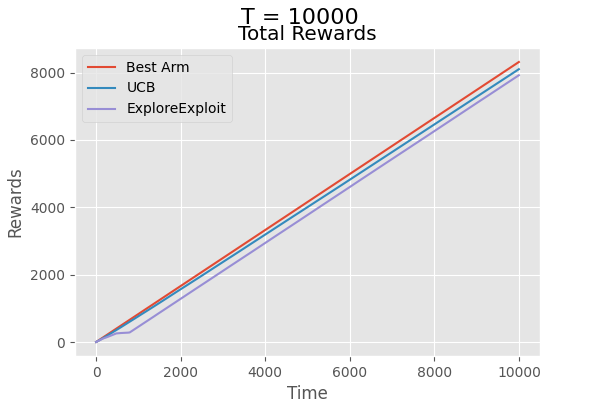
\includegraphics[width=\textwidth]{./Images/plot3.png}
    \end{minipage}
    \caption{Comparison of rewards across different horizons.}
    \label{fig:algorithms_comparison}
\end{figure}

\noindent The results validate UCB’s superiority 
in stochastic Multi-Armed Bandit environments like the one in our problem, 
particularly for large horizons. UCB 
dynamically adjusts exploration, allowing it to focus on high-reward pairs early.
On the other hand Explore \& Exploit 
suffers from a fixed exploration phase, leading to slower adaptation.
Especially for large horizons (like T=10000) UCB likely approaches the theoretical rewards bound,
making it (almost) optimal.
Also, in real-world scenarions where Horizon T is uknown, UCB seems the only choice.



\section*{Subtask 2}
From our lesson we have proven the (instance-dependent) 
theoretical regret bound of UCB:
\[
    E[R(T)] \leq \sum_{i=1}^{K} \frac{8\log(T)}{\Delta_i}
\] 
Since our problem selects pairs of articles $(i,j)$, 
we extend this to all suboptimal pairs.Thus, regret is upper-bounded by:
\[
    E[R(T)] \leq \sum_{j=1}^{K} \sum_{i=1, i \neq j}^{K} \frac{8\log(T)}{\Delta_{(i,j)}}
\]
This extends the single-arm regret bound to our case, where we optimize for pairs instead of single choices.


\section*{Subtask 3}

For subtask 3 we calculate the theoretical regret bound for the UCB algorithm
in our problem.

\begin{figure}[h!]
    \centering
    \begin{minipage}{0.45\textwidth}
        \centering
        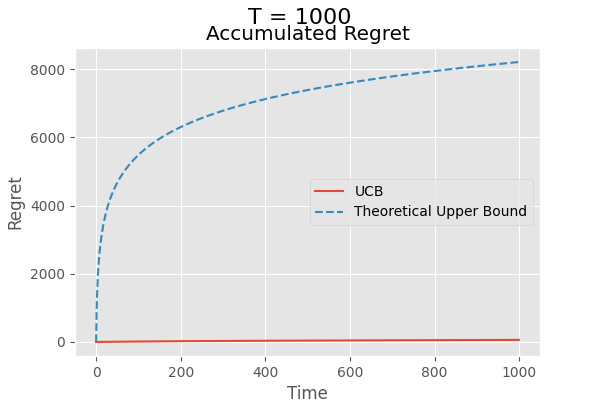
\includegraphics[width=\textwidth]{./Images/plot1.png}
    \end{minipage}\hfill
    \begin{minipage}{0.45\textwidth}
        \centering
        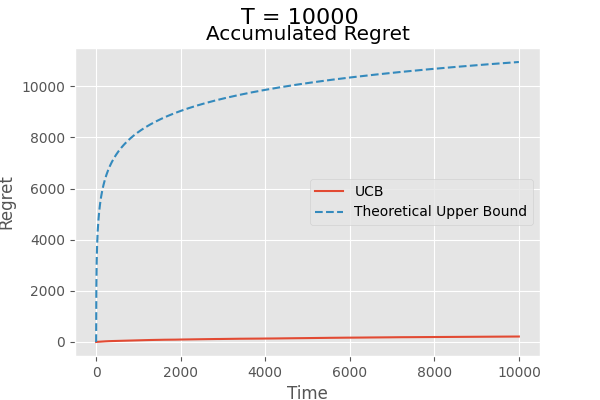
\includegraphics[width=\textwidth]{./Images/plot4.png}
    \end{minipage}
    \caption{Comparison of regret bounds across different horizons.}
    \label{fig:algorithms_comparison}
\end{figure}

\newpage

\noindent In these plot the the theoretical regret curve is significantly 
larger than UCB’s experimental regret at both horizons.
This is expected because theoretical bounds are worst-case guarantees while 
the experimental are instance-dependent.
While the experimental regret appears flat compared to 
the theoretical curve, its growth rate is consistent with logarithmic scaling ($O(\log T)$).
What we can conclude is that the suboptimality gaps ($\Delta_{(i,j)}$)
in this problem instance are, allowing UCB to quickly 
identify and exploit the optimal pair. We can confirm this
by looking at the true probabilities of each arm ($p_1=0.64, p_2=0.45, p_3=
0.53, p_4=0.1, p_5=0.06$). Therefore both grow slower than linear,
indicating the efficiency of UCB. 

\end{document}